% Get excited! - Senku Ishigami

\documentclass[letterpaper, 8pt]{extarticle}
\usepackage{amssymb,amsmath,amsthm,amsfonts}
\usepackage{multicol,multirow}
\usepackage{calc}
\usepackage{ifthen}
\usepackage[landscape]{geometry}
\usepackage[colorlinks=true,citecolor=blue,linkcolor=blue]{hyperref}

\usepackage{booktabs}
\usepackage{ulem}
\usepackage{enumitem}
\usepackage{tabulary}
\usepackage{graphicx}
\usepackage{siunitx}
\usepackage{tikz}
\usepackage{derivative}
\usepackage{svg}
\usepackage{listings}
\usepackage{setspace}
\usepackage{listings}
\usepackage{xcolor}
\usepackage{courier}
\usepackage{syntax}
\usepackage{mathpartir}
\usepackage{siunitx}
\usepackage{physics}

% minimal line spacing
% \setstretch{0.1}

% set borders (experimentally determined to minimize cutoff and maximize space on school printers)
\geometry{top=.25in,left=.25in,right=.25in,bottom=.35in}

% make figures work better in multicol
\newenvironment{Figure}
{\par\medskip\noindent\minipage}
{\endminipage\par\medskip}

\pagestyle{empty} % clear page

% rewrite section commands to be smaller
\makeatletter
\renewcommand{\section}{\@startsection{section}{1}{0mm}%
                                {-1explus -.5ex minus -.2ex}%
                                {0.5ex plus .2ex}%x
                                {\normalfont\normalsize\bfseries}}
\renewcommand{\subsection}{\@startsection{subsection}{2}{0mm}%
                                {-1explus -.5ex minus -.2ex}%
                                {0.5ex plus .2ex}%
                                {\normalfont\small\bfseries}}
\renewcommand{\subsubsection}{\@startsection{subsubsection}{3}{0mm}%
                                {-1ex plus -.5ex minus -.2ex}%
                                {1ex plus .2ex}%
                                {\normalfont\tiny\bfseries}}
\makeatother
\setcounter{secnumdepth}{0} % disable section numbering


% disable indenting
\setlength{\parindent}{0pt}
\setlength{\parskip}{0pt plus 0.5ex}

% Custom siunitx defs
\DeclareSIUnit\noop{\relax}
\NewDocumentCommand\prefixvalue{m}{%
\qty[prefix-mode=extract-exponent,print-unity-mantissa=false]{1}{#1\noop}
}

% Shorthand definitions
\newcommand{\To}{\Rightarrow}
\newcommand{\ttt}{\texttt}
\newcommand{\ra}{\rightarrow}

% condense itemize & enumerate
\let\olditemize=\itemize \let\endolditemize=\enditemize \renewenvironment{itemize}{\olditemize \itemsep0em}{\endolditemize}
\let\oldenumerate=\enumerate \let\endoldenumerate=\endenumerate \renewenvironment{enumerate}{\oldenumerate \itemsep0em}{\endoldenumerate}
\setlist[itemize]{noitemsep, topsep=0pt, leftmargin=*}
\setlist[enumerate]{noitemsep, topsep=0pt, leftmargin=*}

% make matricies narrower
\setlength{\arraycolsep}{2pt}

\title{3SP3}

\begin{document}
\raggedright
\tiny

% make listings look nicer
\lstset{
    tabsize = 2, %% set tab space width
    showstringspaces = false, %% prevent space marking in strings, string is defined as the text that is generally printed directly to the console
    basicstyle = \tiny\ttfamily, %% set listing font and size
    breaklines = true, %% enable line breaking
    numberstyle = \tiny,
    postbreak = \mbox{\textcolor{red}{\(\hookrightarrow\)}\space}
}

\begin{center}
    {\textbf{3SP3 Final - Rocinante Edition}} \\
\end{center}
% set column spacing rules
\setlength{\premulticols}{1pt}
\setlength{\postmulticols}{1pt}
\setlength{\multicolsep}{1pt}
\setlength{\columnsep}{2pt}
\begin{multicols*}{4}
\section{Systems}
\textbf{System}:
Combination of interacting elements organized
to achieve a stated purpose or meet an operational need.
\textbf{System Boundary}:
Defines separation of system of interest and operating environment.
\textbf{Interface}:
Input / Output that flows across system boundaries.
\textbf{Mission}:
A problem that a system intends to solve.
Should be clearly defined by the stakeholder acquiring the system.

\textbf{Life Cycle}
\textbf{Conceptualization}:
Defining requirements.
E.g. what does the market want?
What type of product are we building?
What features do we want?
\textbf{Realization}:
Taking requirements, making design.
Building factories, tooling, prototypes, enter full production.
\textbf{Utilization}:
Processes during the use of the system.
Marketing / sales, maintenance, warranty, recalls, feedback.
\textbf{Retirement}:
End-of-life services.
Recycling, special disposal, updating / disposing of tooling.

\subsection{Systems Engineering}
Top-down approach to design, development, operation of systems.
Iterative, repeats for each lower level until individual elements are defined.
Used because good planning and clear definition of deliverables makes sure that
stakeholder needs and engineering solutions are aligned.

\subsection{Project Life Cycle}
\textbf{Pre-Phase A}:
Concept Studies.
Generate ideas for new missions, draft system concepts.
Establish needs, goals, objectives. Assess feasibility.
\textbf{Phase A}:
Concept and Technology Development.
Develop mission into requirements, system architecture.
Identify technology development required.
\textbf{Phase B}:
Preliminary Design.
Develop system concept into design solution meeting mission needs.
Finish technology development.
\textbf{Phase C}:
Final Design and Fabrication.
Complete detailed design, procure or fabricate components.
Establish procedures, controls for manufacture.
\textbf{Phase D}:
Assembly, Integration, Test, Launch.
Assemble subsystems, integrate,
test to verify and validate system against requirements, deploy.
\textbf{Phase E}:
Operations and Sustainment.
Put system into service.
\textbf{Phase F}:
Closeout.
End of life operations, analysis. Retire system.

\textbf{Stakeholders}:
Groups that are affected or have an interest/stake in program or project.
\textbf{Need}:
A single statement clearly describing what the customer wants.
Domain of customer. Independent of specific solution / implementation.
System is not the need, but response to need.
E.g. ``The Government of Canada needs a more effective means of monitoring shipping traffic in the arctic.''
\textbf{Goals}:
Elaboration of need, setting specific expectations on system.
Qualitative expressions of what system will accomplish.
E.g. ``Provide rapid detection of vessel traffic in Canadian arctic waters.''
\textbf{Objectives}:
Specific target outputs system must achieve.
Specific, Measurable, Attainable, Relevant, Time-Bound.
Quantitative extension of goals.
E.g. ``Detect any surface vessel entering Canadian arctic territorial waters within 1 hour.''
\textbf{Measures of Effectiveness}:
Metrics to judge whether a mission is successful in meeting objectives / achieving goals.
Stated from stakeholder's POV.
E.g. ``No undetected vessels appearing inside 50 nm of Canadian arctic territorial waters.''
(Not directly observable by design team, each MOE assigned 1+ \textit{Measures of Performance},
defining level of perf system must meet to enable MOE.)
\textbf{Constraints}:
Boundaries placed on system design. Usually one of
technical, performance, resources, environmental,
schedule, cost, regulatory, organizational.
\textbf{Concept of Operations}:
Document that outlines high-level vision \& strategy for use \& operation of a system to achieve intended goals.
Who are the stakeholders?
What is the mission?
What is the proposed solution?
How will it be used?
Where will it be used?
By whom?
Over what time?
\textit{Context Diagram}:
Shows mission, system scope.
\textit{Timeline}:
Shows time sequence of operations.
Can identify weak spots, e.g. unacceptable gaps in coverage.
\textbf{Mission Requirements}:
Formal statements defining capabilities, functions, performance, operating condition for system to meet goals, objectives.
Requirements can be validated (demonstrated to be true).
Mission requirements starting point for system requirements.

\section{Requirements}

\section{Launch Environment}

\section{Satellite Systems}

\section{Space Environment}

\section{Math}
\textbf{Dot Product}:
$\vec{a} \cdot \vec{b} = a_x b_x + a_y b_y + a_z b_z = |\vec{a}| |\vec{b}| \cos \theta$;
$|\vec{a}|^2 = \vec{a} \cdot \vec{a}$.
\textbf{Projection}:
$proj_{\vec{b}} \vec{a} = \frac{\vec{a} \cdot \vec{b}}{|\vec{b}|} \frac{\vec{b}}{|\vec{b}|} = \frac{\vec{a} \cdot \vec{b}}{\vec{b} \cdot \vec{b}}\hat{b}$;
$\vec{a}_{\perp \vec{b}} = \vec{a} - proj_{\vec{b}}\vec{a}$.
\textbf{Cross Product}:
$\vec{a} \times \vec{b} = (a_y b_z - a_z b_y)\hat{i} - (a_x b_z - a_z b_x)\hat{j} + (a_x b_y - a_y b_x)\hat{k}$;
$\hat{n}_{ab} = \frac{\vec{a} \times \vec{b}}{|\vec{a} \times \vec{b}|}$;
$\vec{a} \times \vec{b} = |a| |b| \sin \theta \hat{n}_{ab}$.

\section{Orbital Mechanics}
% TODO: see if i'm missing anything here
\subsection{2D}
\textbf{Kepler's Laws}
K1 - Orbit of planet is ellipse, Sun at one of two foci.
K2 - Line segment joining planet, Sun sweeps out equal areas during equal intervals of time.
K3 - Square of planet's orbital period proportional to cube of length of semi-major axis of orbit.

\subsubsection{Forces}
$\vec{F} = m \vec{a} = \odv{\vec{p}}{t}$.
$\vec{p} = m \vec{v}$.
\textbf{Impulse on mass $m$:}
$I = \int_{t_1}^{t_2} \vec{F} \dd{t} = m \vec{v}_2 - m \vec{v}_1$.
$\Delta \vec{v} = I / m = F_{net} \Delta t / m$ (if $F_{net}$ const).
\textbf{Gravitational Constant:}
$G = 6.67430 \times 10^{-11} \, \frac{\text{Nm}^2}{\text{kg}^2}$.

\subsubsection{Rotation, Torque, Angular Momentum}
\textbf{Torque (moment) on mass m:} $\vec{M_0} = \vec{r} \times \vec{F} = \odv{\vec{H_0}}{t}$
\textbf{Angular Momentum:} $\vec{H_0} = \vec{r} \times m \vec{v} = \vec{r} \times \vec{p}$

\subsubsection{Orbits}

\textbf{Two-body equation of motion:}
$\mu = G(m_1 + m_2)$ (gravitational param);
$\ddot{\vec{r}} = -\frac{G(m_1 + m_2)}{r^3} \vec{r} = - \frac{\mu}{r^3}\vec{r}$.

\textbf{Angular Momentum:} $\vec{h} = \vec{r} \times \vec{v}$ \si{\kilo\gram\metre\per\second} (convert to \si{\kilo\gram\kilo\metre\per\second} if needed)

\textbf{Eccentricity vector}: $\vec{e} = \frac{\vec{C}}{\mu}$
\textbf{Orbit Equation}:
$\boxed{r = \frac{h^2}{mu} \frac{1}{1 + e \cos \theta}}$

\subsubsection{Circular Orbit $e = 0$}
$r = h^2 / \mu = \mu / v^2$;
$h = r v_\perp$;
$v = v_\perp$;
$v_{circ} = \sqrt{\frac{\mu}{r}}$;
$T_{circ} = \frac{2 \pi}{\sqrt{mu} r^{3/2}}$

\subsubsection{Orbital Constants}
$G = 6.67430 \times 10^{-20}$ \si{\newton\kilo\metre\squared\per\kilo\gram\squared};
$R_E = 6378$ \si{\kilo\metre};
$M_E = 5.97219 \times 10^{24}$ \si{\kilo\gram};
$\mu = G(M_e + M_s) \approx G(M_e) \approx 398600$ \si{\kilo\metre\cubed\per\second\squared};

\subsubsection{Elliptical Orbit $0 < e < 1$}
$r = \frac{h^2}{\mu} \frac{1}{1 + e \cos \theta} = \frac{a (1 - e^2)}{1 + e \cos \theta}$. \\
\textbf{Periapsis}: Closest approach. \\
\textbf{Apoapsis}: Furthest approach. $a + c$ away from the mass at focal point. \\
\textbf{Semimajor axis}: $a = \frac{h^2}{\mu} \frac{1}{1 - e^2}$ (the longer one) \\
\textbf{Semiminor axis}: $b = a \sqrt{1 - e^2}$ (the shorter one) \\
\textbf{Linear eccentricity}: $c = a e$ \\
\textbf{Semilatus rectum}: $p = \frac{h^2}{\mu}$ \\
\textbf{True anomaly}: $\theta$, the degree of rotation from periapsis. \\
\textbf{Specific Energy of $m2$ (constant)}: $\epsilon = -\frac{1}{2} \frac{\mu}{h^2}(1 - e^2)$. \\
\textbf{Orbit Period}: $T_{ellipse} = \frac{2 \pi a b}{h} = \frac{2 \pi a^{3/2}}{\sqrt{\mu}}$, \\
where $b = a \sqrt{1 - e^2}, h = \sqrt{\mu a(1-e^2)}$ \\

\subsubsection{Parabolic Trajectory $e = 1$, Hyperbolic Trajectory $e > 1$}
$v_{esc} = \sqrt{2} v_{circ}$, arrive at inifinity with 0 velocity.
$v_\infty^2 = v^2 - v_{esc}^2$, arrive at inifinity with velocity $v_\infty$.

\subsubsection{Perifocal Frame}
Coordinate frame where orbit lies in XY plane.
\begin{itemize}
    \item Centered at the focus
    \item X axis points along apse line to periapsis (0 true anomaly)
    \item Y axis along semilatus rectum
    \item Z axis in normal direction of angular momentum $\vec{\mathbf{h}}$
\end{itemize}

$r = \frac{h^2}{\mu} \frac{1}{1 + e \cos(\theta)},
x = r \cos \theta, y = r \sin \theta
$

$\vec{\mathbf{r}} = x \, \hat{\mathbf{p}} + y \, \hat{\mathbf{q}}$

$\vec{\mathbf{r}} = \frac{h^2}{\mu} \frac{1}{1 + e \cos(\theta)} 
\left( \cos(\theta) \, \hat{\mathbf{p}} + \sin(\theta) \, \hat{\mathbf{q}} \right)$

$\vec{\mathbf{v}} = \dot{x} \, \hat{\mathbf{p}} + \dot{y} \, \hat{\mathbf{q}}$

$\vec{\mathbf{v}} = \frac{\mu}{h} 
\left( -\sin(\theta) \, \hat{\mathbf{p}} + (e + \cos(\theta)) \, \hat{\mathbf{q}} \right)$

\subsubsection{Orbit Relationships}
$2a = r_a + r_p$;
$e = \frac{r_a - r_p}{r_a + r_p}, \frac{r_p}{r_a} = \frac{1-e}{1+e}$;
$a = \frac{h^2}{\mu} \frac{1}{1 - e^2}$;
$h = \sqrt{\mu a (1 - e^2)} = r_a v_{\perp a} = r_p v_{\perp p}$;

$r_a = \frac{h^2}{\mu} \frac{1}{1-e}$;
$r_p = \frac{h^2}{\mu} \frac{1}{1+e}$;

$v_\perp = \frac{\mu}{h}(1 + e \cos \theta)$
$v_r = \frac{\mu}{h} e \sin \theta$


\subsubsection{Orbit Energy}

\subsubsection{Lagrange Coefficients}
$h = |\vec{r_0} \times \vec{v_0}|$;
$v_{r0} = \vec{v_0} \cdot \frac{\vec{r_0}}{r_0}$;
$r = \frac{h^2}{\mu} \frac{1}{1 + \left(\frac{h^2}{\mu r_0} - 1\right) \cos(\Delta \theta) - h \frac{v_{r0}}{\mu} \sin(\Delta \theta)}$

$f = 1 - \frac{\mu r}{h^2} (1 - \cos(\Delta \theta)), g = \frac{r r_0}{h} \sin(\Delta \theta)$ \\
$\dot{f} = \frac{\mu}{h} \frac{1 - \cos(\Delta \theta)}{\sin(\Delta \theta)} \left[\frac{\mu}{h^2} (1 - \cos(\Delta \theta)) - \frac{1}{r_0} - \frac{1}{r}\right]$
$\dot{g} = 1 - \frac{\mu r_0}{h^2} (1 - \cos(\Delta \theta))$

\textbf{Therefore,}
$\vec{r} = f \vec{r_0} + g \vec{v_0}$;
$\vec{v} = \dot{f} \vec{r_0} + \dot{g} \vec{v_0}$

Solving for eccentricity, initial true anomaly:
$r_0 = \frac{h^2}{\mu} \frac{1}{1 + e \cos(\theta_0)}$
$v_{r0} = \frac{\mu}{h} e \sin(\theta_0)$

\subsubsection{Orbit Position as a Function of Time}
Circle:
$\theta(t) = \frac{\mu^2}{h^3} t, t(\theta) = \frac{h^3}{\mu^2} \theta$

Elliptical Orbit:
$M_e = t \frac{\mu^2}{h^3} (1 - e^2)^{3/2}$\\
$E = 2 \tan^{-1} \left(\sqrt{\frac{1 - e}{1 + 3}} \tan(\frac{\theta}{2})\right)$\\
$e \sin E = \frac{e \sqrt{1 - e^2} \sin(\theta)}{1 + e \cos(\theta)}$\\
$M_e = E - e \sin E = \frac{2 \pi t}{T_{orbit}}$\\
(given $\theta$ solve for $t$ directly, or $\theta \to E \to M_e \to t$)

\subsection{3D}
\textbf{Sidereal Rate:} Rotation rate of Earth relative to ``fixed stars'',
$\omega_E = 7.292115 \times 10^{-5}$ \si{rad\per\second}.
\textbf{Right Ascention:} Degrees east along equator from vernal equinox.
\textbf{Declination:} Latitude north from equator.

\subsubsection{Geocentric Equatorial Frame}
Coordinate frame is fixed, used to rep satellite position, velocity.
\textbf{X axis} along direction of vernal equinox (at chosen epoch!)
\textbf{Z axis} along Earth's axis of rotation (at chosen epoch!)
\textbf{Y axis} completes cartesian coordinate system.
Precession, Nutation of the Earth spin axis causes it to drift over time, so epoch matters.
(Precession: Earth's axis rotating around a central axis, Nutation: variations / wiggles in precession)

\subsubsection{Orbital Parameters}
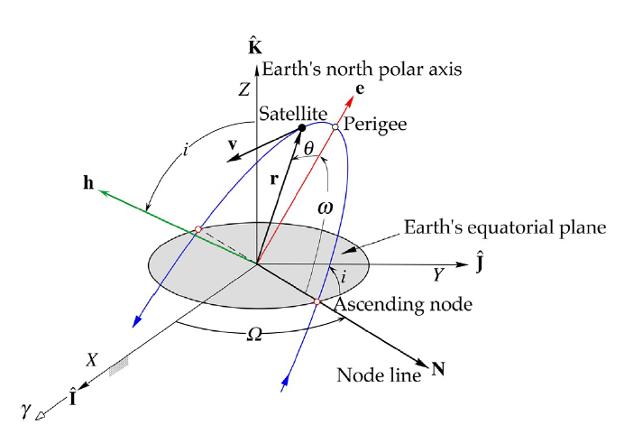
\includegraphics[width=\linewidth]{3D Orbital Parameters.png}
Given Position and Velocity vectors, we can calculate orbital elements:

\begin{enumerate}
    \item Distance: $r = \sqrt{\vec{r} \cdot \vec{r}}$
    \item Speed: $v = \sqrt{\vec{v} \cdot \vec{v}}$
    \item Radial velocity: $v_r = \frac{\vec{r}}{r} \cdot \vec{v}$
          ($v_r > 0$ away from perigee, $v_r < 0$ towards perigee)
    \item Specific angular momentum: $\vec{h} = \vec{r} \times \vec{v}$
          (magnitude $h = \sqrt{\vec{h} \cdot \vec{h}}$)
    \item Inclination: $i = \cos^{-1} (h_Z / h)$
        ($0^\circ \leq i < 90^\circ$: prograde orbit (same direction as Earth rotation),
        $90^\circ < i \leq 180^\circ$: retrograde orbit (opposite direction to Earth rotation))
    \item Node line: $\vec{N} = \hat{K} \times \vec{h}$
        (Magnitude $N = \sqrt{\vec{N} \cdot \vec{N}}$)
    \item RAAN: $\Omega = \cos^{-1} (N_X / N)$
        ($N_Y \geq 0, \Omega = \cos^{-1} (N_X / N)$,
        $N_Y < 0, \Omega = 360^\circ - \cos^{-1}(N_X / N)$)
    \item Eccentricity vector: $\vec{e} 
        = \frac{\vec{v} \times \vec{h}}{\mu} - \frac{\vec{r}}{r}
        = \frac{1}{\mu} \left[\left(v^2 - \frac{\mu}{r}\right) \vec{r} - r v_r \vec{v}\right]$
        (Magnitude: $e = \sqrt{\vec{e} \cdot \vec{e}}$)
    \item Argument of perigee: $\omega = 
    \begin{cases}
        e_Z \geq 0 & \cos^{-1} \left(\frac{\vec{N}}{N} \cdot \frac{\vec{e}}{e}\right) \\
        e_Z < 0 & 360^\circ - \cos^{-1} \left(\frac{\vec{N}}{N} \cdot \frac{\vec{e}}{e}\right) \\
    \end{cases}$
    \item True Anomaly: $\theta =
    \begin{cases}
        v_r \geq 0 & \cos^{-1} \left(\frac{\vec{e}}{e} \cdot \frac{\vec{r}}{r}\right) \\
                   & \text{or } \cos^{-1} \left(\frac{1}{e} \left[\frac{h^2}{\mu r} - 1\right]\right) \\
        v_r < 0    & 360^\circ - \cos^{-1} \left(\frac{\vec{e}}{e} \cdot \frac{\vec{r}}{r}\right) \\
                   & \text{or } 360^\circ - \cos^{-1} \left(\frac{1}{e} \left[\frac{h^2}{\mu r} - 1\right]\right) \\
    \end{cases}$
\end{enumerate}

\subsubsection{Perifocal to ECI Frame}

$
\vec{\mathbf{r}} = \frac{h^2}{\mu} \frac{1}{1 + e \cos(\theta)} 
\begin{bmatrix}
\cos(\theta) \\
\sin(\theta) \\
0
\end{bmatrix}
$

$
\vec{\mathbf{v}} = \frac{\mu}{h}
\begin{bmatrix}
- \sin(\theta) \\
e + \cos(\theta) \\
0
\end{bmatrix}
$

\subsubsection{2D Rotations}

\subsubsection{3D Rotations}

\textbf{Euler Z-X-Z:}
$
(\alpha, \beta, \gamma) \to R_Z(\gamma) R_X{\beta} R_Z(\alpha)
\mid \alpha \in [0^\circ, 360^\circ], \beta \in [0, 180^\circ], \gamma \in [0^\circ, 360^\circ]
$

$
\vec{v}_{x' y' z'} =
\begin{bmatrix}
    \cos \gamma & \sin \gamma & 0 \\
    -\sin \gamma & \cos \gamma & 0 \\
    0 & 0 & 1
\end{bmatrix}
\begin{bmatrix}
    1 & 0 & 0 \\
    0 & \cos \beta & \sin \beta \\
    0 & -\sin \beta & \cos \beta \\
\end{bmatrix}
\begin{bmatrix}
    \cos \alpha & \sin \alpha & 0 \\
    -\sin \alpha & \cos \alpha & 0 \\
    0 & 0 & 1 \\
\end{bmatrix}
\vec{v}_{xyz}
$

$Q_{ZXZ} =$
% scalebox abuse to get this to fit
\scalebox{0.85}{$
\begin{bmatrix}
-\sin\alpha \cos\beta \sin\gamma + \cos\alpha \cos\gamma & \cos\alpha \cos\beta \sin\gamma + \sin\alpha \cos\gamma & \sin\beta \sin\gamma \\
-\cos\alpha \cos\beta \sin\gamma - \cos\alpha \sin\gamma & \cos\alpha \cos\beta \cos\gamma - \sin\alpha \sin\gamma & \sin\beta \cos\gamma \\
\sin\alpha \sin\beta & -\cos\alpha \sin\beta & \cos\beta
\end{bmatrix}
$}

\textbf{Yaw-Pitch-Roll:}
$
(\alpha, \beta, \gamma) \to R_X(\gamma) R_Y(\beta) R_Z(\alpha)
\mid \alpha \in [0, 360^\circ], \beta \in (-90^\circ, 90^\circ), \gamma \in [0^\circ, 360^\circ]
$

$
\vec{v}_{x' y' z'}
= \begin{bmatrix}
    1 & 0 & 0 \\
    0 & \cos \gamma & \sin \gamma \\
    0 & -\sin \gamma & \cos \gamma \\
\end{bmatrix}
\begin{bmatrix}
    \cos \beta & 0 & -\sin \beta \\
    0 & 1 & 0 \\
    \sin \beta & 0 \cos \beta \\
\end{bmatrix}
\begin{bmatrix}
    \cos \alpha & \sin \alpha & 0 \\
    -\sin \alpha & \cos \alpha & 0 \\
    0 & 0 & 1
\end{bmatrix}
$
$
\vec{v}_{xyz}
$

$
Q_{YPR} =
$
\scalebox{0.85}{$
\begin{bmatrix}
\cos\alpha \cos\beta & \sin\alpha \cos\beta & -\sin\beta \\
\cos\alpha \sin\beta \sin\gamma - \sin\alpha \cos\gamma & \sin\alpha \sin\beta \sin\gamma + \cos\alpha \cos\gamma & \cos\beta \sin\gamma \\
\cos\alpha \sin\beta \cos\gamma + \sin\alpha \sin\gamma & \sin\alpha \sin\beta \cos\gamma - \cos\alpha \sin\gamma & \cos\beta \cos\gamma
\end{bmatrix}
$}

\textbf{Perifocal to Geocentric Equatorial}
$
Q_{GCE \to pfc} = R_Z(\omega) R_X(i) R_Z(\Omega)
$
$
Q_{pfc \to GCE} = Q_{XYZ \to pqw}^T = R_Z(-\Omega) R_X(-i) R_Z(-\omega) =
$
\scalebox{0.8}{$
\begin{bmatrix}
    -\sin\omega \cos i \sin\Omega + \cos\omega \cos\Omega & -\cos\omega \cos i \sin\Omega - \sin\omega \cos\Omega & \sin i \sin\Omega \\
    \cos\omega \cos i \sin\Omega + \cos\omega \sin\Omega & \cos\omega \cos i \cos\Omega - \sin\omega \sin\Omega & -\sin i \cos\Omega \\
    \sin\omega \sin i & \cos\omega \sin i & \cos i
\end{bmatrix}
$}

\subsubsection{Oblateness}
\textbf{Regression of Node:}
$
\dot{\Omega} = -\left[
    \frac{3}{2} \frac{\sqrt{\mu} J_2 R^2}{(1 - e^2)^2 a^{7/2}}
\right] \cos i
$

\textbf{Advance of Perigee:}
$
\dot{\omega} = -\left[
    \frac{3}{2} \frac{\sqrt{\mu} J_2 R^2}{(1 - e^2)^2 a^{7/2}}
\right]
\left(
    \frac{5}{2} \sin^2 i - 2
\right)
$

\section{Satellite Communications}

\section{Satellite Attitude \& Orbit Control Systems}

\section{Spacecraft Dynamics}

\end{multicols*}

\end{document}
